\begin{figure}[h]
    \centering
    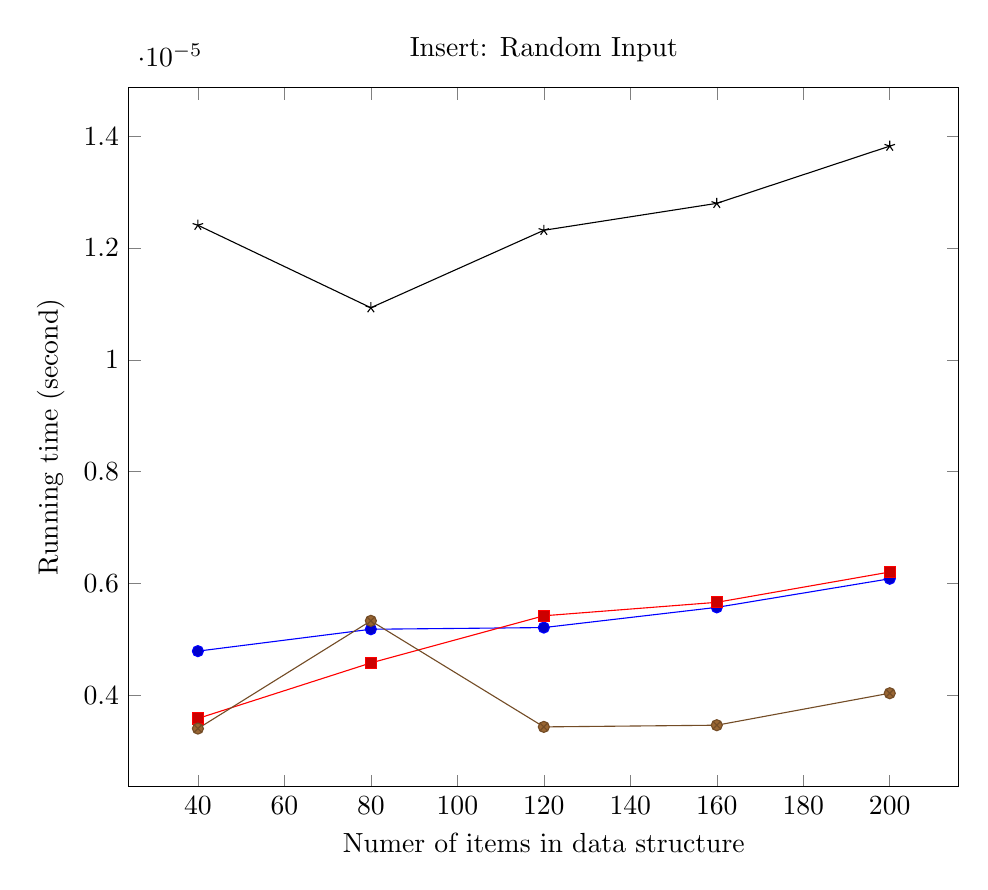
\begin{tikzpicture}
        \begin{axis}[
            xlabel={Numer of items in data structure},
            ylabel={Running time (second)},
            title={Insert: Random Input},
            width=\textwidth
        ]
		\addplot coordinates {
			(200, 6.083741802384579e-06)
			(160, 5.571743729905488e-06)
			(120, 5.2103333258043946e-06)
			(80, 5.180215792129072e-06)
			(40, 4.78868785435127e-06)
		};
		\addplot coordinates {
			(200, 6.2042119370830925e-06)
			(160, 5.662096330932842e-06)
			(120, 5.421156061530263e-06)
			(80, 4.577865118624014e-06)
			(40, 3.583986507343928e-06)
		};
		\addplot coordinates {
			(200, 4.035749512473763e-06)
			(160, 3.463516372642639e-06)
			(120, 3.4333988389673165e-06)
			(80, 5.3308034605042964e-06)
			(40, 3.4032813052947695e-06)
		};
		\addplot coordinates {
			(200, 1.3823947956900785e-05)
			(160, 1.2799951811948152e-05)
			(120, 1.2318071273142995e-05)
			(80, 1.0932664724086494e-05)
			(40, 1.2408423874168962e-05)
		};
        \legend{}
        \end{axis}
    \end{tikzpicture}
    \caption{Average of 0 operations, benchmarked every 0, starting at 0.}
\end{figure}